\documentclass[
a4paper,
cleardoublepage=empty,
headings=twolinechapter,
numbers=autoenddot,
]{scrbook}
\setcounter{secnumdepth}{4}
\usepackage[italian]{babel}
\usepackage{amsmath}
\usepackage{amsfonts}
\usepackage{amssymb}
\usepackage[signatures,swapnames,sans]{frontespizio}
\usepackage{todonotes}
\usepackage{verbatim}
\usepackage{graphicx} %LaTeX package to import graphics
\graphicspath{image/} %configuring the graphicx package,le immagini si trovano in image/
\usepackage{hyperref}
\usepackage{float}
\usepackage[utf8]{inputenc}
\usepackage[T1]{fontenc}
\usepackage{cite}
\usepackage{url}
\title{Ambliopia}
\author{Luca Frangiamore}
\pagestyle{plain}
\date{2023}
\begin{document}
	
	\frontmatter
	
	\pdfbookmark{Title page}{titlepage}
	
	\begin{frontespizio}
		\Margini{3cm}{3cm}{3cm}{3cm}
		\Universita{Bergamo}
     	\Logo[43.332mm]{image/Marchio}
		\Divisione{Scuola di Ingegneria}
		\Corso[Laurea Triennale]{Ingegneria Informatica\\Classe n. L-8 Ingegneria dell’informazione (D.M. 270/04)}
		\Titolo{Ambliopia}
		\Punteggiatura{}
		\NCandidato{Tesi di Laurea Triennale}
		\Candidato[1074443]{Frangiamore Luca}
		\Relatore{Prof.\ Angelo Gargantini}
		\Annoaccademico{2022--2023}
		
	\end{frontespizio}
	
	\tableofcontents
	\listoffigures
	\mainmatter
	
	
	\chapter*{Introduzione}
	Nel corso della seguente trattazione, andrò a descrivere il processo che mi ha portato alla realizzazione di un gioco mobile all'interno del progetto 3D4Amb, condotto dall'Università di Bergamo e diretto dal professore Angelo Gargantini. L'obiettivo del progetto è quello di creare applicazioni innovative per la diagnosi e la cura dell'ambliopia, una patologia visiva che colpisce principalmente i bambini e che consiste in una riduzione dell'acuità visiva di un occhio, che non riesce a lavorare correttamente a causa di un problema nella trasmissione dei segnali visivi al cervello.
	
	In particolare, il progetto 3D4Amb si prefigge di utilizzare la tecnologia 3D e gli strumenti di realtà virtuale per la creazione di applicazioni interattive che stimolino la visione dell'occhio pigro, sfruttando supporti fisici per differenziare le immagini dirette ai rispettivi occhi. L'obiettivo finale è quello di fornire una soluzione innovativa e personalizzata per la diagnosi e la cura dell'ambliopia, che possa essere utilizzata sia in ambito clinico che a casa.\\\\
	
	Nel primo capitolo, approfondirò il problema dell'occhio pigro, descrivendone i sintomi e i possibili trattamenti, evidenziando l'importanza di una diagnosi precoce e della cura della patologia per prevenire conseguenze a lungo termine. \\\\
	Nel secondo capitolo, descriverò il progetto 3D4Amb, illustrando gli strumenti e i supporti utilizzati per la creazione delle applicazioni, evidenziando l'importanza dell'innovazione tecnologica per la diagnosi e la cura dell'ambliopia.\\\\
	
	Nel terzo capitolo, mi concentrerò sulla descrizione dettagliata del flusso di lavoro che mi ha portato alla realizzazione del gioco mobile all'interno del progetto, evidenziando i problemi incontrati e le soluzioni adottate per superarli.\\\\
	
	Infine, nell'ultimo capitolo, le conclusioni, esprimerò le mie considerazioni sul progetto e le possibili migliorie future per sviluppare soluzioni ancora più efficaci per la diagnosi e la cura dell'ambliopia.
	
	\chapter{Ambliopia}
	L'ambliopia, anche conosciuta come "occhio pigro" è una patologia che si manifesta nei primi anni dello sviluppo, età compresa tra 0-6 anni, il quale colpisce circa il 4\% della popolazione mondiale\cite{perc_amblipia}.
	La patologia riguarda la non corretta stimolazione dell'apparato visivo, in questo caso il cervello non riesce a ricreare l'immagine tridimensionale e quindi per evitare il fenomeno della visione doppia, anche detta \textbf{diplopia}, il cervello tenterà di sopprimere un immagine.
	Nella maggior parte dei casi, l'occhio è anatomicamente perfetto, \textbf{ambliopia funzionale}, in casi peggiori possiamo riscontrare \textbf{ambliopia organica} in cui vi è una deviazione delle vie ottiche.
	La seguente patologia si può manifestare con più probabilità in maniera asimmetrica, \textbf{monolaterale}, la quale colpisce un solo occhio, o più raramente possiamo trovare la forma \textbf{bilaterale}, la quale colpisce entrambi gli occhi.
	Normalmente l'ambliopia non peggiora durante la vita adulta in quanto oramai lo sviluppo alterato della vista si è oramai instaurato, l'età in cui l'ambliopia si stabilizza in modo permanente va dagli 8 ai 15 anni.
	\section{Diagnosi}
	La diagnosi è un punto fondamentale per il trattamento dell'ambliopia, in quanto, una diagnosi tardiva può influire negativamente sulla corretta terapia, riducendo le possibilità di recupero.
	Il trattamento in genere viene personalizzata dal medico oculistico.
	\begin{itemize}
		\item Classica, in cui si cerca di stabilire l'acuità visiva e la visione binoculare del piccolo paziente. In caso di strabismo sarà necessaria anche una visita ortottica, la quale è una branca dell'oftalmologia che si occupa della valutazione e riabilitazione di deficit muscolari e sensoriali.
		\item Pediatric Vision Scanner, Negli ultimi anni si sta sviluppando un nuovo metodo in grado di riconoscere l'ambliopia in età pediatrica con alta precisione, figura:\ref{fig:pvs}.
		Come pubblicato nell'articolo Validation of the Pediatric Vision Scanner in a normal preschool population\cite{pvs}, in cui si prende in esame Pediatric Vision Scanner(PVS), il quale scatta una foto ad entrambi gli occhi per poi andare a misurare errore di rifrazione e disallineamento.
		\begin{figure}[h]
			\centering
			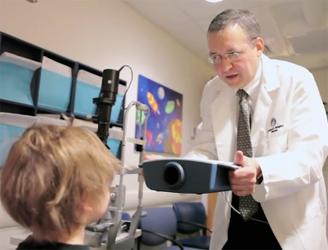
\includegraphics[width=0.7\linewidth]{image/pvs}
			\caption{Pediatric Vision Scanner.Fonte:\cite{PVS_image}}
			\label{fig:pvs}
		\end{figure}\\
		Il metodo in questione, descritto nell'articolo sopra citato, ha permesso di identificare correttamente tutti e 6 i bambini con ambliopia e/o strabismo nel campione di 300 bambini, garantendo così una precisione del 100\%. Inoltre, il metodo potrebbe essere in grado di diagnosticare l'ambliopia già a partire dai 2 anni di età, suggerendo un potenziale miglioramento nella diagnosi precoce di questa patologia.
		
	\end{itemize}
	
	\section{Cause}
	In generale come detto prima, l'occhio pigro riguarda il progressivo trascuramento dei segnali di uno dei due occhi.
	Questo processo di sviluppo è causato da un non corretto sviluppo delle vie nervose degli occhi, le quali vengono stimolate in modo non bilanciate, ciò è dovuto magari dalla presenza di una condizione oculare presente in uno dei due occhio.
	Alcune condizioni che possono insorgere sono:
	\begin{itemize}
		\item Astigmatismo, visione poco nitida e distorta in qualsivoglia direzione.
		\item Strabismo, deviazione degli assi visivi, impedisce il corretto coordinamento degli occhi. 
		\item Cataratta, opacizzazione parziale o totale del cristallino,  causa affaticamento e difficoltà nel mettere a fuoco le immagini.
		\item Ptosi palpebrale, una o entrambe le palpebre superiori sono abbassate più del normale.
	\end{itemize}
	Come detto prima, se il cervello non riesce a combinare le immagini provenienti dai due occhi, esso può decidere di trascurare un dei due segnali, prediligendo l'occhio ottimale, sviluppando quindi l'ambliopia.
	\section{Sintomi}
	Tra i problemi più comuni causati dall'ambliopia, oltre alla ridotta acuità visiva dell'occhio colpito, ci sono:
	
	\begin{itemize}
		\item Scarsa percezione della profondità: l'ambliopia può ridurre la capacità di percepire la profondità poiché la coordinazione visiva tra i due occhi viene compromessa.
		\item Difficoltà di visione in un occhio, l'ambliopia può causare la soppressione dell'occhio colpito dal cervello, il che può portare a problemi di visione come la riduzione della percezione del contrasto, della percezione dei colori e della visione notturna.
		\item Movimenti involontari dell'occhio, l'ambliopia può causare movimenti oculari anormali, come lo strabismo, che a loro volta possono causare diplopia (visione doppia).
		\item Sensibilità al movimento compromessa, i pazienti affetti da ambliopia possono avere difficoltà a distinguere il movimento e possono essere più sensibili al movimento nell'occhio non colpito.
	\end{itemize}
	È importante diagnosticare e trattare l'ambliopia il prima possibile, poiché il trattamento è più efficace durante l'infanzia e l'adolescenza. In generale, il trattamento dell'ambliopia prevede l'uso di occhiali, l'occlusione dell'occhio sano per stimolare la vista dell'occhio pigro e la terapia visiva.
	\section{Trattamenti}
	Subito dopo aver riconosciuto il disturbo bisogna procedere con la corretta terapia.Come prima cosa, bisogna correggere il difetto che ha portato l'inibizione dell'occhio pigro, successivamente si procede con le terapie.
	\begin{itemize}
		\item Patching\cite{patching}, La terapia consiste nel coprire l'occhio dominante, da applicare per un periodo di tempo variabile, figura:\ref{fig:patching}.
		Il trattamento è efficacie, ma il recupero della vista impiega diversi mesi.       	   
		\begin{figure}[H]
			\centering
			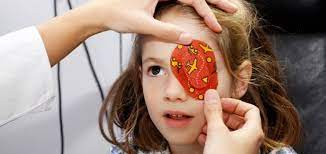
\includegraphics[width=0.5\linewidth]{image/patching}
			\caption{Trattamento con Patching.Fonte:\cite{Patching_image}}
			\label{fig:patching}
		\end{figure}	
		\item Collirio, permette di offuscare la vista dell'occhio dominante, in modo da poter stimolare l'occhio più debole
		\item Lenti opacizzazione, usate per limitare la visione dell'occhio sano e stimolare l'occhio pigro a lavorare di più, figura:\ref{fig:penalizzazione-ottica}. Un articolo che ha esaminato gli effetti delle lenti di Bangerter sulla funzione binoculare in pazienti con ambliopia è The effect of Bangerter filters on binocular function in observers with amblyopia\cite{filtro}.
		\begin{figure}[h]
			\centering
			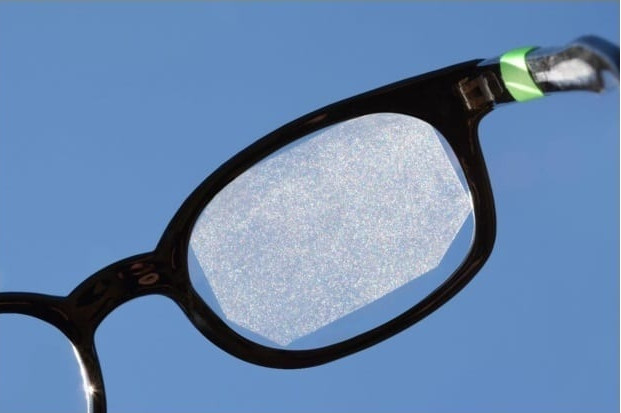
\includegraphics[width=0.4\linewidth]{image/penalizzazione ottica}
			\caption{Trattamento con lente di bangerter.
				Fonte:\cite{Bangerter_image}}
			\label{fig:penalizzazione-ottica}
		\end{figure}
		
		
		
		\item Pattern Flicker\cite{Pattern-Flicker}, è costituito da una cupola semisferica nera contenente un ottagono di LED rossi e una console utilizzata per controllare i LED stessi, figura:\ref{fig:Pattern-Flicker}.
		\begin{figure}[H]
			\centering
			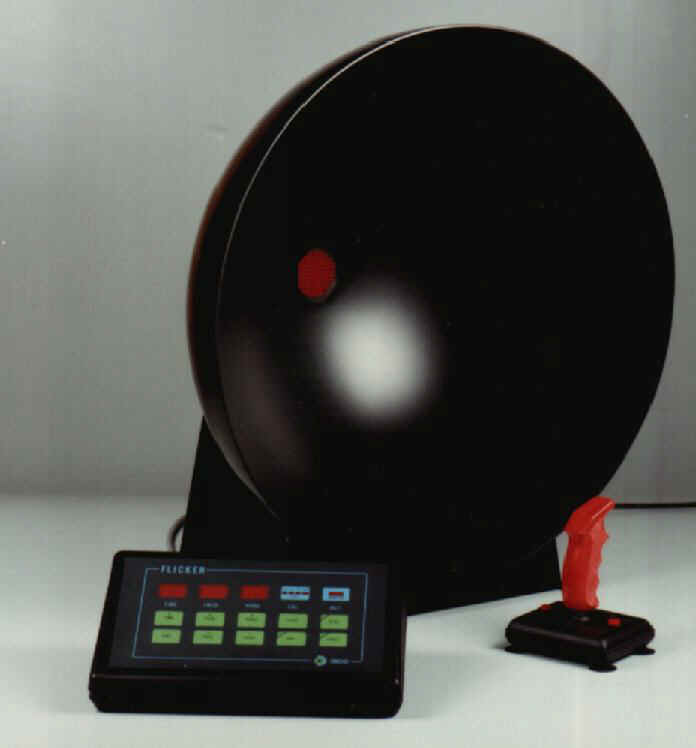
\includegraphics[width=0.4\linewidth]{image/Pattern_Flicker}
			\caption{Pattern Flicker.Fonte:\cite{Pattern-Flicker}}
			\label{fig:Pattern-Flicker}
		\end{figure}
		L'utilizzo di luci a LED rosse a bande alternate rappresenta una forma di stimolazione mirata e interattiva per migliorare l'efficienza visiva dei bambini. Questo tipo di trattamento, effettuato su uno sfondo nero per evitare distrazioni, mira a bombardare in modo mirato e selettivo i fotorecettori dell'occhio per stimolare i nervi ottici. Tuttavia, è importante sottolineare che questo trattamento potrebbe non essere adatto per pazienti epilettici in quanto può scatenare crisi
		\item Esiste poi un altro tipo di tecnologia, I-BiT Plus\cite{I-Bit}, il quale permette al paziente di intrattenersi mediante giochi interattivi o video.
		Il suo funzionamento si basa sul mostrare la parte più "interessante" del gioco, come ostacoli o obiettivi all'occhio pigro, mentre all'occhio sano vengono mostrati oggetti di contorno, come i paesaggi.
		Per assicurare che il paziente continui a guardare le immagini in un posizione ottimale il sistema si serve di un Eye tracker, in modo da garantire il corretto posizionamento dell'immagine.
		\item Luminopia, è un software approvato da \textbf{Food and Drug Administration(FDA)}\cite{Approvazione_luminopia} come annunciato dal CEO Scott Xiao, che permette ai pazienti di poter usufruire di 700 ore di serie o film, adattati tramite AI. Questo sistema permette di rendere il trattamento dell'ambliopia piacevole e quindi sopportabile nel lungo periodo.
		I pazienti usufruiscono di questi contenuti mediante il vr, in modo da poter visionare i contenuti scelti.
	
		\item AmblyoPlay, è un innovativo sistema facilmente accessibile tramite tablet o qualsiasi altro supporto elettronico, che offre una serie di giochi che possono essere utilizzati per 30 minuti al giorno. Per utilizzare il software è necessario possedere gli occhiali AmblyoPlay, degli occhiali anaglifici, capitolo:\ref{chap:occhiali_anaglifici} che permettono di differenziare due immagini sovrapposte. Questo sistema offre una serie di esercizi utili per migliorare 6 abilità visive fondamentali, figura:\ref{fig:6 abilità}, migliorando la quindi la vista in generale.
    	\begin{figure}[H]
			\centering
			\includegraphics[width=0.5\linewidth]{image/6 abilità}
			\caption{Abilità visive fondamentali.Fonte:\cite{amblyoplay}}
			\label{fig:6 abilità}
     	\end{figure}
		\item Film, Il metodo proposto per trattare l'ambliopia consiste nella visione di filmati in 3D con l'utilizzo di occhiali polarizzati e l'applicazione di una maschera digitale su un occhio e l'inversa su quello sano, figura:\ref{fig:film}, permettendo di combinare le informazioni dei due occhi per percepire un'immagine completa. La forma e la posizione delle maschere cambiano ogni 10 secondi, e se il paziente riesce a percepire l'immagine completa, il contrasto dell'occhio sano viene aumentato nella sessione successiva. 
		\begin{figure}[H]
			\centering
			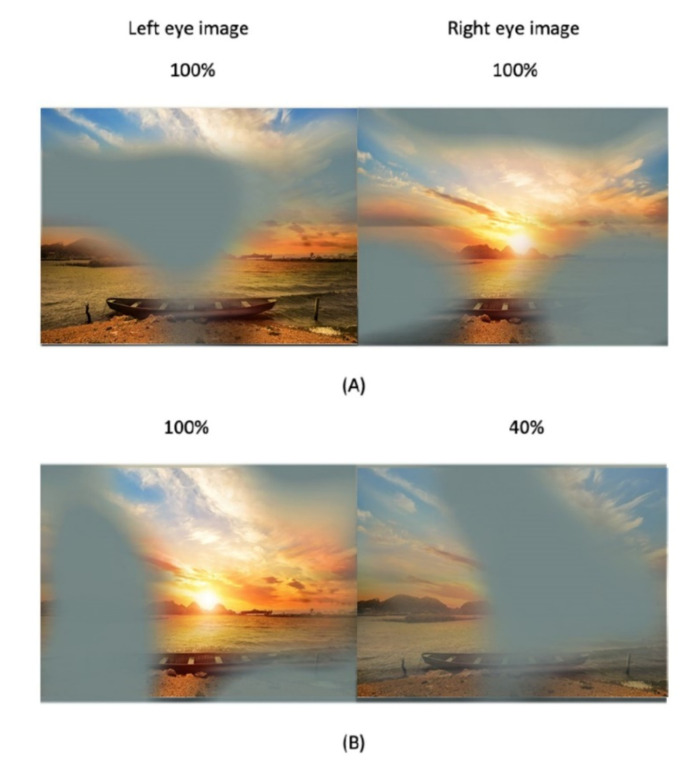
\includegraphics[width=0.5\linewidth]{image/filmAmblio}
			\caption{Esempio maschera.Fonte:\cite{nuoviTrattamenti}}
			\label{fig:film}
		\end{figure}
	    Questo metodo rappresenta un'alternativa per i pazienti con grave ambliopia che non possono giocare ai videogiochi.
	    \item Il Diplopia Game, è un videogioco per computer che viene eseguito sull'Oculus Rift OC DK2. il gioco consiste in diversi livelli, figura:\ref{fig:vivid} in cui i soggetti devono usare entrambi gli occhi per catturare oggetti, distruggere blocchi e completare obiettivi. Lo studio di Ziak et al. ha dimostrato un miglioramento medio di 1,5 linee logMAR nell'acuità visiva di soggetti affetti da ambliopia anisometropica dopo 8 sessioni di gioco.
	    \begin{figure}[H]
	    	\centering
	    	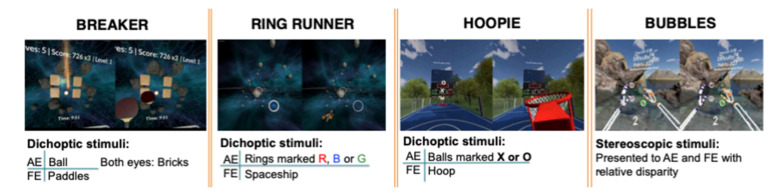
\includegraphics[width=0.9\linewidth]{image/vivid}
	    	\caption{Giochi proposti.Fonte:\cite{nuoviTrattamenti}}
	    	\label{fig:vivid}
	    \end{figure}
	    \item Dig Rush, è un gioco d'avventura ad azione che si gioca su iPad con occhiali anaglifi, capitolo:\ref{chap:occhiali_anaglifici}. Il gioco consiste nel fare scavare dei minatori per trovare l'oro e riportarlo al carro, evitando ostacoli come fuoco, lava e mostri. L'occhio ambliope vede gli elementi a contrasto elevato, mentre l'altro occhio vede gli elementi a basso contrasto. Per avere successo nel gioco, entrambi gli occhi devono vedere i rispettivi elementi del gioco. È stato dimostrato che il gioco ha un effetto positivo sul trattamento dell'ambliopia infantile ed è stato più efficace del patching dopo due settimane di utilizzo. Tuttavia, sarebbe consigliabile utilizzarlo per un periodo più lungo.
	    \begin{figure}[H]
	    	\centering
	    	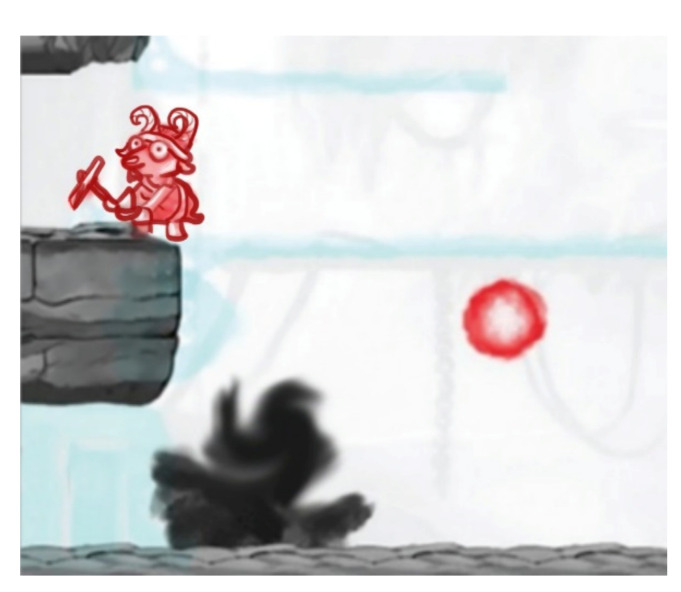
\includegraphics[width=0.5\linewidth]{image/dig rush}
	    	\caption{Schermata di gioco.Fonte:\cite{nuoviTrattamenti}}
	    	\label{fig:dig_rush}
	    \end{figure}
	
	\end{itemize}
	
	\chapter{3D4Amb}
    Il progetto è stato creato con l'intenzione di creare uno strumento utile ed economico per il trattamento e la misurazione dell'occhio pigro, basato sulla tecnologia 3D..
	\begin{figure}[h]
		\centering
		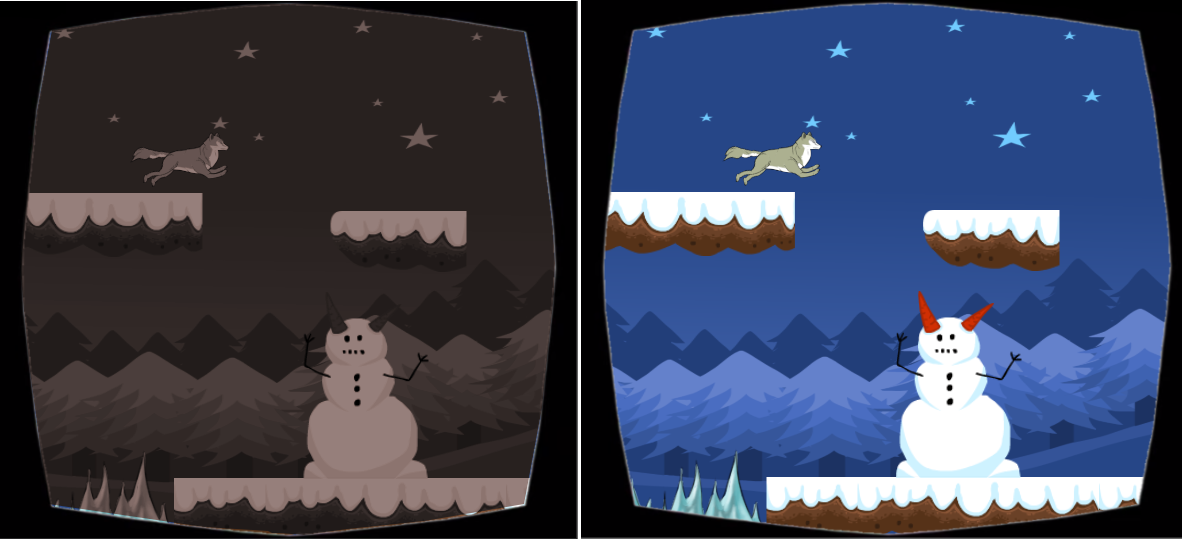
\includegraphics[width=0.8\linewidth]{image/3D4Amb}
		\caption{Logo 3D4Amb.Fonte:\cite{3d4amb}}
		\label{fig:3D4Amb}
	\end{figure}
	\section{Funzionamento e strumenti}
	Il funzionamento di base del sistema 3D4Amb consiste nel presentare al paziente due immagini correlate tra loro ma leggermente diverse, pre-elaborate tramite il software 3D4Amb. Questo permette di creare una percezione tridimensionale della scena, dando la sensazione che gli oggetti si trovino davanti ai propri occhi.
	Per realizzare le applicazioni videoludiche basate sulla differenziazione delle immagini, 3D4Amb utilizza diversi supporti tecnologici, il tutto a basso costo
	Per garantire il corretto sdoppiamento, sono state sperimentate diverse soluzioni. Una di queste è l'utilizzo di occhiali speciali dotati di lenti polarizzate, che permettono ai due occhi di vedere immagini diverse, in base alla polarizzazione delle lenti. Un'altra soluzione consiste nell'utilizzo di schermi speciali, che proiettano due immagini diverse in modo che ciascun occhio possa vederne una sola.
	Inoltre, per garantire la massima efficienza del sistema, è importante considerare anche la distanza tra gli occhi del paziente, in modo da regolare il sistema di visualizzazione in base alle caratteristiche anatomiche di ciascun individuo. In questo modo, è possibile ottenere una visione tridimensionale più nitida e confortevole per il paziente.
	\subsection{Cardboard}\label{chap:cardboard}
	Il funzionamento del Google Cardboard, figura:\ref{fig:cardboard}, si basa sulla creazione di un effetto stereoscopico\cite{Stereoscopio}, utilizzando uno smartphone, il quale viene inserito all'interno del dispositivo.
	Il cardboard utilizza due lenti che ingrandiscono l'immagine fino a riempire il campo visivo\cite{Funzionamento_cardboard}.
	\begin{figure}[H]
		\centering
		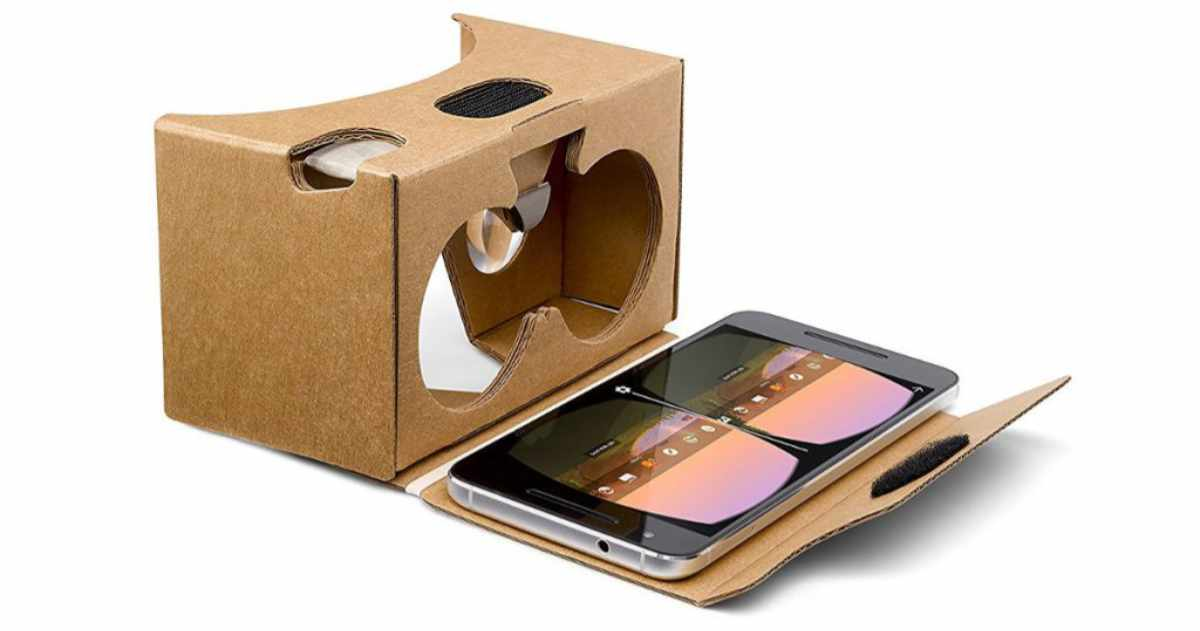
\includegraphics[width=0.8\linewidth]{image/cardboard}
		\caption{Cardboard di cartone.Fonte:\cite{Cardboard_image}}
		\label{fig:cardboard}
	\end{figure}
	Questo dispositivo ci permette di poter usufruire della tecnologia 3D con un costo relativamente basso, che si aggira sui 10\$, esso ci permette di mostrare immagini completamente diverse ai due occhi.
	\begin{figure}[H]
		\centering
		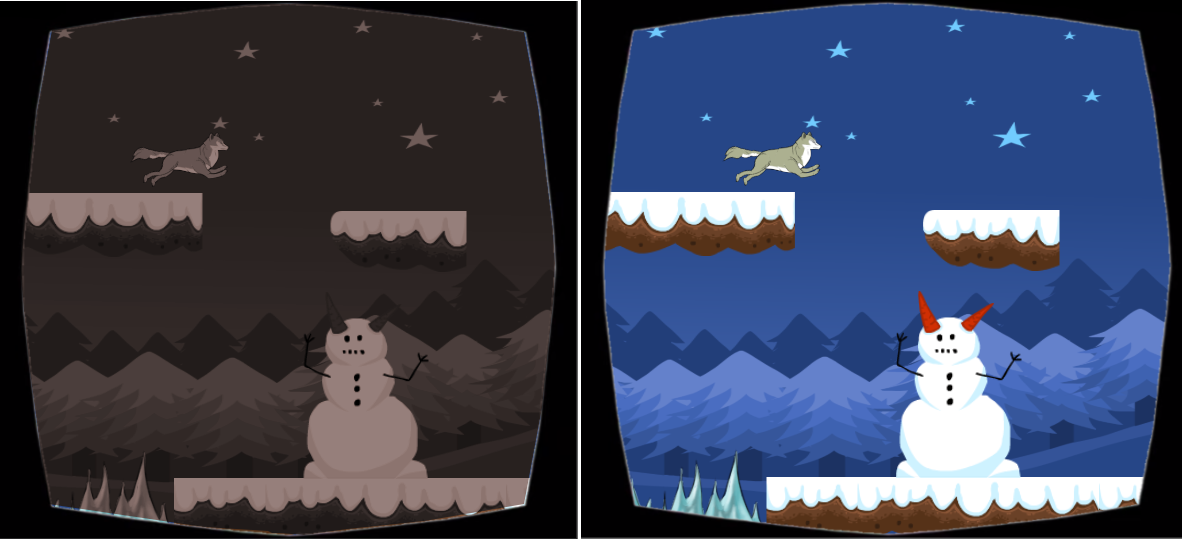
\includegraphics[width=0.8\linewidth]{image/3D4Amb_1}
		\caption{Differenziazione colori.
			Fonte:\cite{3d4amb}}
		\label{fig:cardboard-3D4Amb_colori}
	\end{figure}
	Come mostrato nella figura:\ref{fig:cardboard-3D4Amb_colori}, le immagini mostrate differisco per il colore, vi sono casi in cui si può andare ad omettere un elemento della scena, figura:\ref{fig:cardboard-3D4Amb_elementi}
	\begin{figure}[H]
		\centering
		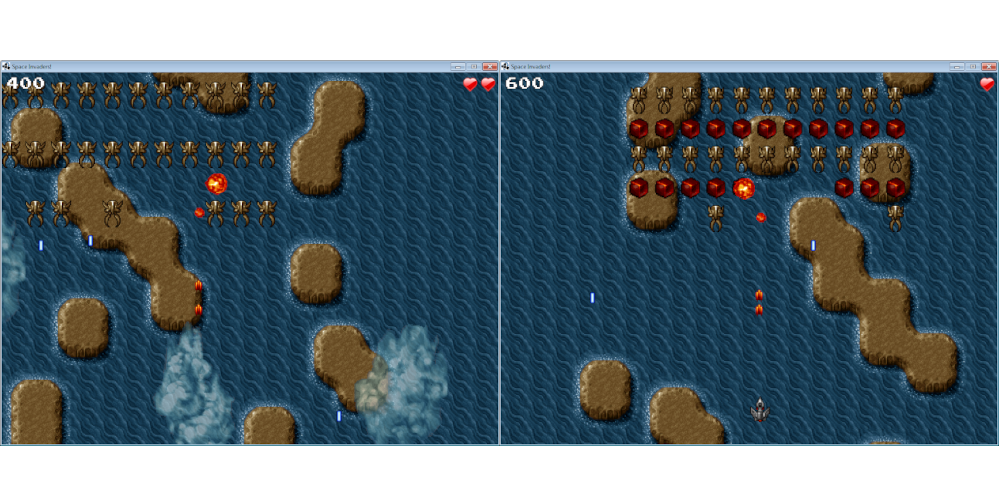
\includegraphics[width=0.8\linewidth]{image/3D4Amb_2}
		\caption{Differenziazione elementi su schermo.Fonte:\cite{3d4amb}}
		\label{fig:cardboard-3D4Amb_elementi}
	\end{figure}
	Il cardboard è uno strumento di realtà virtuale a basso costo che sfrutta il proprio smartphone come schermo e processore. Questo significa che, grazie al cardboard, è possibile sfruttare tutte le potenzialità del proprio smartphone per creare esperienze di realtà virtuale. Inoltre, il fatto che il telefono risieda all'interno del cardboard permette di dividere le immagini emesse dallo schermo del telefono in modo che siano percepite come immagini separate dai due occhi, creando un effetto di tridimensionalità e immersività per l'utente. Grazie a questa tecnologia, è possibile accedere a un'ampia gamma di applicazioni di realtà virtuale disponibili sullo store del proprio smartphone, rendendo l'esperienza di realtà virtuale accessibile a un pubblico sempre più vasto.
	\subsection{Occhiali Anaglifici}\label{chap:occhiali_anaglifici}
	Gli occhiali anaglifici, come si può vedere nella figura \ref{fig:occhiali_anaglifici}, sono provvisti da due lenti in gelatina rossa e ciano, dette anche filtri, che vengono utilizzati per permettere all'occhio di percepire un'immagine composta da due immagini sovrapposte, ognuna delle quali filtrata da un colore diverso. In particolare, una delle due immagini è filtrata in rosso e l'altra in ciano, in modo che quando l'immagine viene vista attraverso le lenti degli occhiali, ciascun occhio vede solo l'immagine che gli corrisponde e il cervello le unisce per creare l'effetto tridimensionale. Questa tecnica, chiamata anaglifo, è stata utilizzata per la visione di immagini tridimensionali fin dagli anni '50, e ancora oggi viene utilizzata in alcune applicazioni di realtà virtuale e giochi in 3D.
	\begin{figure}[H]
		\centering
		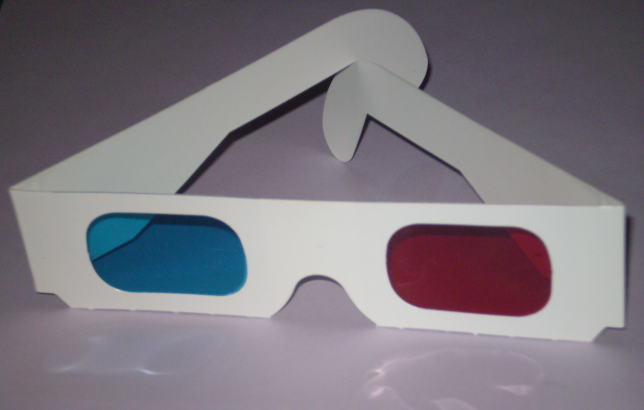
\includegraphics[width=0.6\linewidth]{image/occhiali_anaglifici}
		\caption{occhiali anaglifici.Fonte:\cite{Anaglifo_image}}
		\label{fig:occhiali_anaglifici}
	\end{figure}
	Le immagini sono distanti tra loro(generalmente 5,7 cm), con colori complementari, figura:\ref{fig:anaglifo}, essi vengono usati per poter osservare solo l'immagine cromatica complementare, questo permette di ricreare l'effetto tridimensionale.
	\begin{figure}[H]
		\centering
		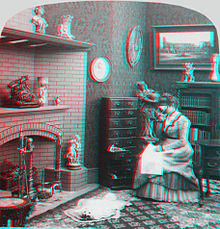
\includegraphics[width=0.6\linewidth]{image/anaglifo}
		\caption{Anaglifo.Fonte:\cite{Anaglifo_image}}
		\label{fig:anaglifo}
	\end{figure}
	
	\subsection{Active shutter 3D system}
	L'active shutter 3D system, invece, utilizza degli occhiali attivi, dotati di lenti liquide o cristalli liquidi che si alternano rapidamente tra uno stato di trasparenza e uno di opacità per bloccare la visione di uno degli occhi mentre l'altro vede l'immagine corrispondente, a una frequenza che può arrivare anche a 120Hz. In questo modo, le immagini vengono mostrate in rapida successione alternando i due occhi, creando la sensazione di visione tridimensionale. Questa tecnologia è diversa rispetto a quella del cardboard, in cui le immagini sono mostrate contemporaneamente davanti a entrambi gli occhi.
	\begin{figure}[H]
		\centering
		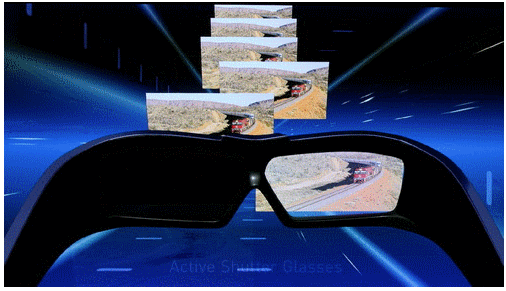
\includegraphics[width=0.6\linewidth]{image/active-shutter-3d-technology}
		\caption{Differenziazione elementi su schermo.Fonte:\cite{active-shutter-3d_image}}
		\label{fig:occhiali active-shutter-3d-technology}
	\end{figure}
	
	\section{Obiettivi}
	Il progetto 3D4Amb è stato concepito con l'intento di sviluppare un sistema avanzato basato sulla tecnologia 3D, mirato a migliorare la diagnosi e il trattamento dell'ambliopia nei bambini piccoli. Grazie all'uso di immagini tridimensionali differenti per ciascun occhio, il sistema consente una diagnosi più precisa e semplice dell'ambliopia, che può poi essere trattata attraverso l'impiego di giochi interattivi e attività di intrattenimento.
	\begin{itemize}
		\item Basso costo, in modo che possa essere acquistato da famiglie di qualsiasi estrazione economica. A tal fine, si è scelto di basare il sistema su tecnologie facilmente reperibili e accessibili al pubblico, che richiedono un investimento economico limitato.
		\item Semplice da usare, in quanto non richiede alcuna formazione specifica e può essere utilizzato dai bambini con una supervisione limitata o nulla. Si mira, inoltre, a rendere il sistema adatto all'uso domestico, evitando la necessità di recarsi in ospedale o in centri specializzati.
		\item Estendibile, grazie all'impiego di tecnologie standard e, possibilmente, open source, il sistema è progettato per consentire a sviluppatori terzi di ampliare le funzionalità in modo semplice e immediato. Ciò garantisce la massima flessibilità e scalabilità del sistema nel tempo, in modo da poterlo adattare alle esigenze dei singoli utenti e alle future evoluzioni del mercato.
	\end{itemize}
	In definitiva, il progetto 3D4Amb rappresenta un'importante opportunità per migliorare la qualità della vita dei bambini affetti da ambliopia, garantendo loro un trattamento innovativo, efficace e accessibile a tutti.
	
	\chapter{Progetto}
	L'obiettivo di questa tesi è quello di sviluppare uno strumento di terapia per l'ambliopia che sia in grado di intrattenere maggiormente il paziente. Per raggiungere questo obiettivo, ho implementato un videogioco utilizzando il cardboard per sdoppiare le immagini. Il genere scelto è FPS (First Person Shooter), in modo da costringere il paziente a osservare e girare l'ambiente circostante in modo dettagliato, cosa che sarebbe stata più difficile da realizzare mediante altri generi. L'utilizzo del cardboard ha reso il gioco più immersivo e coinvolgente. Inoltre, ho scelto di utilizzare dei toni fanciulleschi per alleggerire il più possibile la terapia. L'intento ludico del gioco risiede nel fattore di progressione tra i vari livelli, che al momento sono 3. Per l'interazione con l'ambiente, ho deciso di utilizzare un gamepad, come mostrato in figura \ref{fig:gamepad}, il quale mi permette di avere un buon numero di tasti e di conseguenza maggiori possibilità di interazione con il gioco.
	\begin{figure}[H]
		\centering
		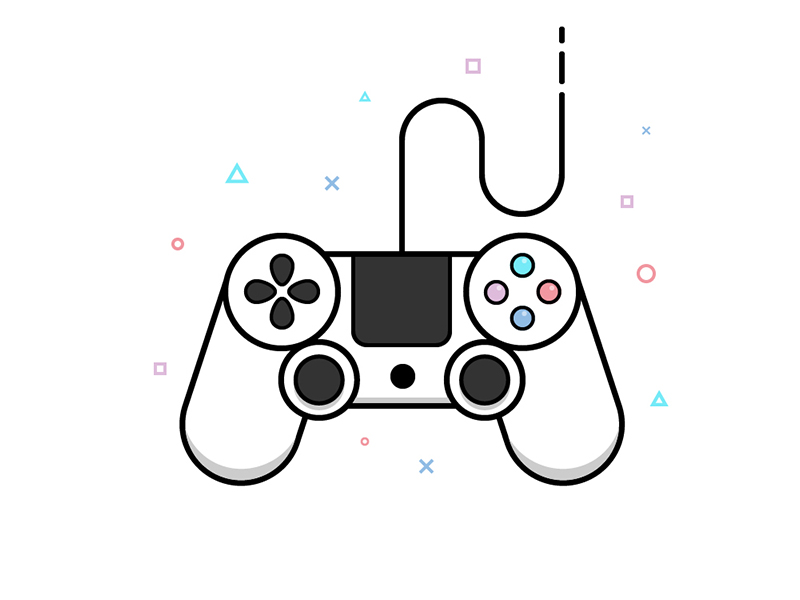
\includegraphics[width=0.8\linewidth]{image/gamepad}
		\caption{Layout gamepad utilizzato.Fonte:\cite{controller_image}}
		\label{fig:gamepad}
	\end{figure}
	\section{Struttura}
	La struttura dell'applicativo è molto lineare, bisogna raccogliere dei punti mediante l'interazione con determinati oggetti sparsi per la mappa, denominati Target, una volta fatto ciò, si procede al livello successivo.
	Ogni livello è caratterizzato da un grado di trasparenza diverso, argomento che verrà trattato maggiormente nei paragrafi successivi.
	I livelli di trasparenza sono 3:
	\begin{enumerate}
		\item Facile
		\item Medio
		\item Difficile
	\end{enumerate}
	La struttura dei livelli è molto lineare, in diversi punti della mappa vi sono diversi obiettivi a cui bisogna sparare, ogni Target permette al paziente di ottenere dei punti, dopo aver ottenuto un determinato punteggio si aprirà un portale che condurrà al livello successivo.
	Al interno dei livelli vi sono degli oggetti denominati \textit{OcchioMalato}, i quali verranno mostrati trasparenti all'occhio sano e solidi a quello pigro, come nella figura:\ref{fig:pozzo}. 
	\begin{figure}[H]
		\centering
		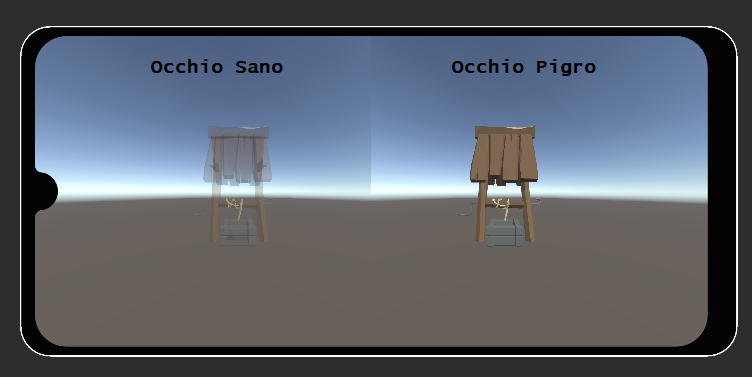
\includegraphics[width=0.8\linewidth]{image/Pr_trasparenza}
		\caption{Esempio di trasparenza mediante un oggetto di gioco}
		\label{fig:pozzo}
	\end{figure}
	Nella figura \ref{fig:pozzo}, possiamo notare come ai due occhi venga mostrato lo stesso oggetto ma con diversa trasparenza, in questo modo sollecitiamo l'occhio afflitto da ambliopia, lasciando anche una traccia all'occhio sano.
	Il livello di trasparenza aumenterà(gli oggetti diventano più trasparenti) man mano che si avanzerà di livello, in modo da poter stimolare efficacemente l'occhio con il passare dei livelli.
	\subsection{Target}
	Per questo progetto i Target sono utilizzati per rendere l'esperienza più ludica, dando al paziente un obiettivo da portare a termine, con difficoltà crescente, in modo da rendere il tutto più sopportabile per il lungo periodo.
	I Target sono principalmente degli scudi medievali, figura:\ref{fig:target_score}, i quali sono sparsi all'interno dei vari livelli di gioco.
	\begin{figure}[H]
		\centering
		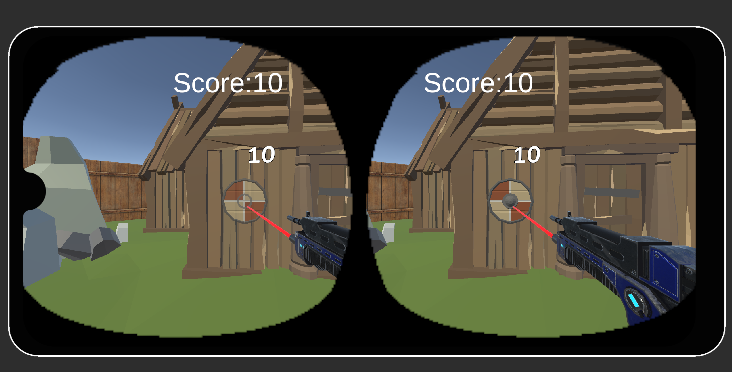
\includegraphics[width=0.7\linewidth]{image/target_score}
		\caption{Target con punteggio}
		\label{fig:target_score}
	\end{figure}
	Essi si possono trovare in 2 forme:
	\begin{itemize}
		\item Scudo Classico, mostrato in figura:\ref{fig:target_score}, in questo caso la difficoltà risiede nel loro posizionamento.
		\item Scudo in Movimento, mostrato in figura:\ref{fig:target_movimento}, caratterizzato dal fatto che l'obiettivo è in movimento, costringendo quindi il paziente a muovere lo sguardo.
	\end{itemize}
	\begin{figure}[H]
		\centering
		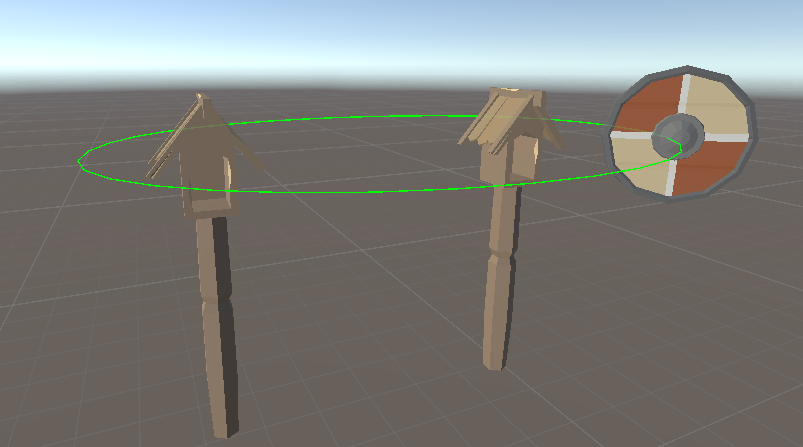
\includegraphics[width=0.7\linewidth]{image/target_movimento}
		\caption{Target in movimento}
		\label{fig:target_movimento}
	\end{figure}
	\section{Tecnologie utilizzate}
	Nell'era moderna, le tecnologie disponibili sono diverse, per la realizzazione del progetto mi sono avvalso delle seguenti tecnologie:
	\begin{itemize}
		\item:Cardboard, 
		\item:Unity 3D, motore di gioco
		\item:Visual Code, editor di codice sorgente
	\end{itemize}
	\subsection{Cardboard, motivi della scelta}\label{chap:cardboard_motivi}
	La motivazione che mi ha portato a scegliere il cardboard e non gli occhiali anaglifici risiedono principalmente nella sua versatilità, visto che mi permette di poter realizzare un'applicazione con limitati limiti tecnici e con un budget ridotto, fatto cruciale, visto che si parla principalmente di un'applicazione idealmente indirizzata per pazienti giovanissimi, i quali potranno usufruire dei sui benefici comodamente da casa.
	Una delle tecnologie che mi è stata particolarmente utile è il giroscopio del telefono, che risiede all'interno del cardboard. Questo componente mi ha permesso di creare un'esperienza di immersione più avanzata, in quanto, ha reso possibile la percezione del movimento e dell'orientamento spaziale del dispositivo, trasferendo queste informazioni nel gioco. Grazie al giroscopio, figura:\ref{fig:giroscopio}, il giocatore può ruotare la visuale all'interno dell'ambiente virtuale semplicemente inclinando e/o ruotando la testa, senza dover utilizzare nessunaltro dispositivo di controllo. Questo ha reso l'esperienza di gioco più fluida e naturale, aumentando l'immersione del paziente nell'ambiente virtuale e rendendo il gioco ancora più coinvolgente.
	\begin{figure}[H]
		\centering
		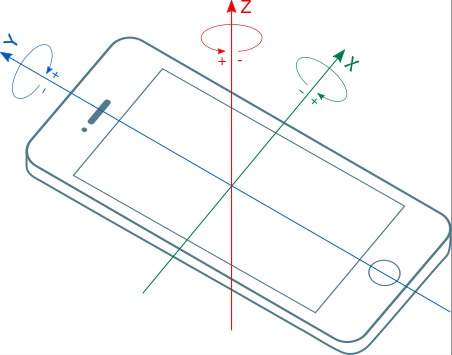
\includegraphics[width=0.5\linewidth]{image/giroscopio}
		\caption{Assi Giroscopio.Fonte:\cite{Giro_image}}
		\label{fig:giroscopio}
	\end{figure}
	\subsection{Unity 3D}\label{unity3D}
	Unity 3D è un motore di gioco sviluppato dalla Unity
	Technologies, il quale permette di realizzare dei videogiochi tridimensionali e bidimensionali, la sua community e le varie guide messe a disposizione da unity permettono di cimentarsi in questo progetto superando il plateau di apprendimento.
	Si tratta di uno strumento che permette di alleggerire il processo di produzione attraverso l'utilizzo di un'interfaccia grafica ben organizzata, vi sono 4 schermate principali:
	\begin{itemize}
		\item Scene, Permette di spostare e/o modificare gli oggetti nella scena.
		\item Simulator, Permette di eseguire l'applicativo.
		\item Inspector, Il quale mette a disposizione delle impostazioni di modifica.
		\item Hierarchy, Mostra i vari elementi nella scena.
	\end{itemize}
	\begin{figure}[H]
		\centering
		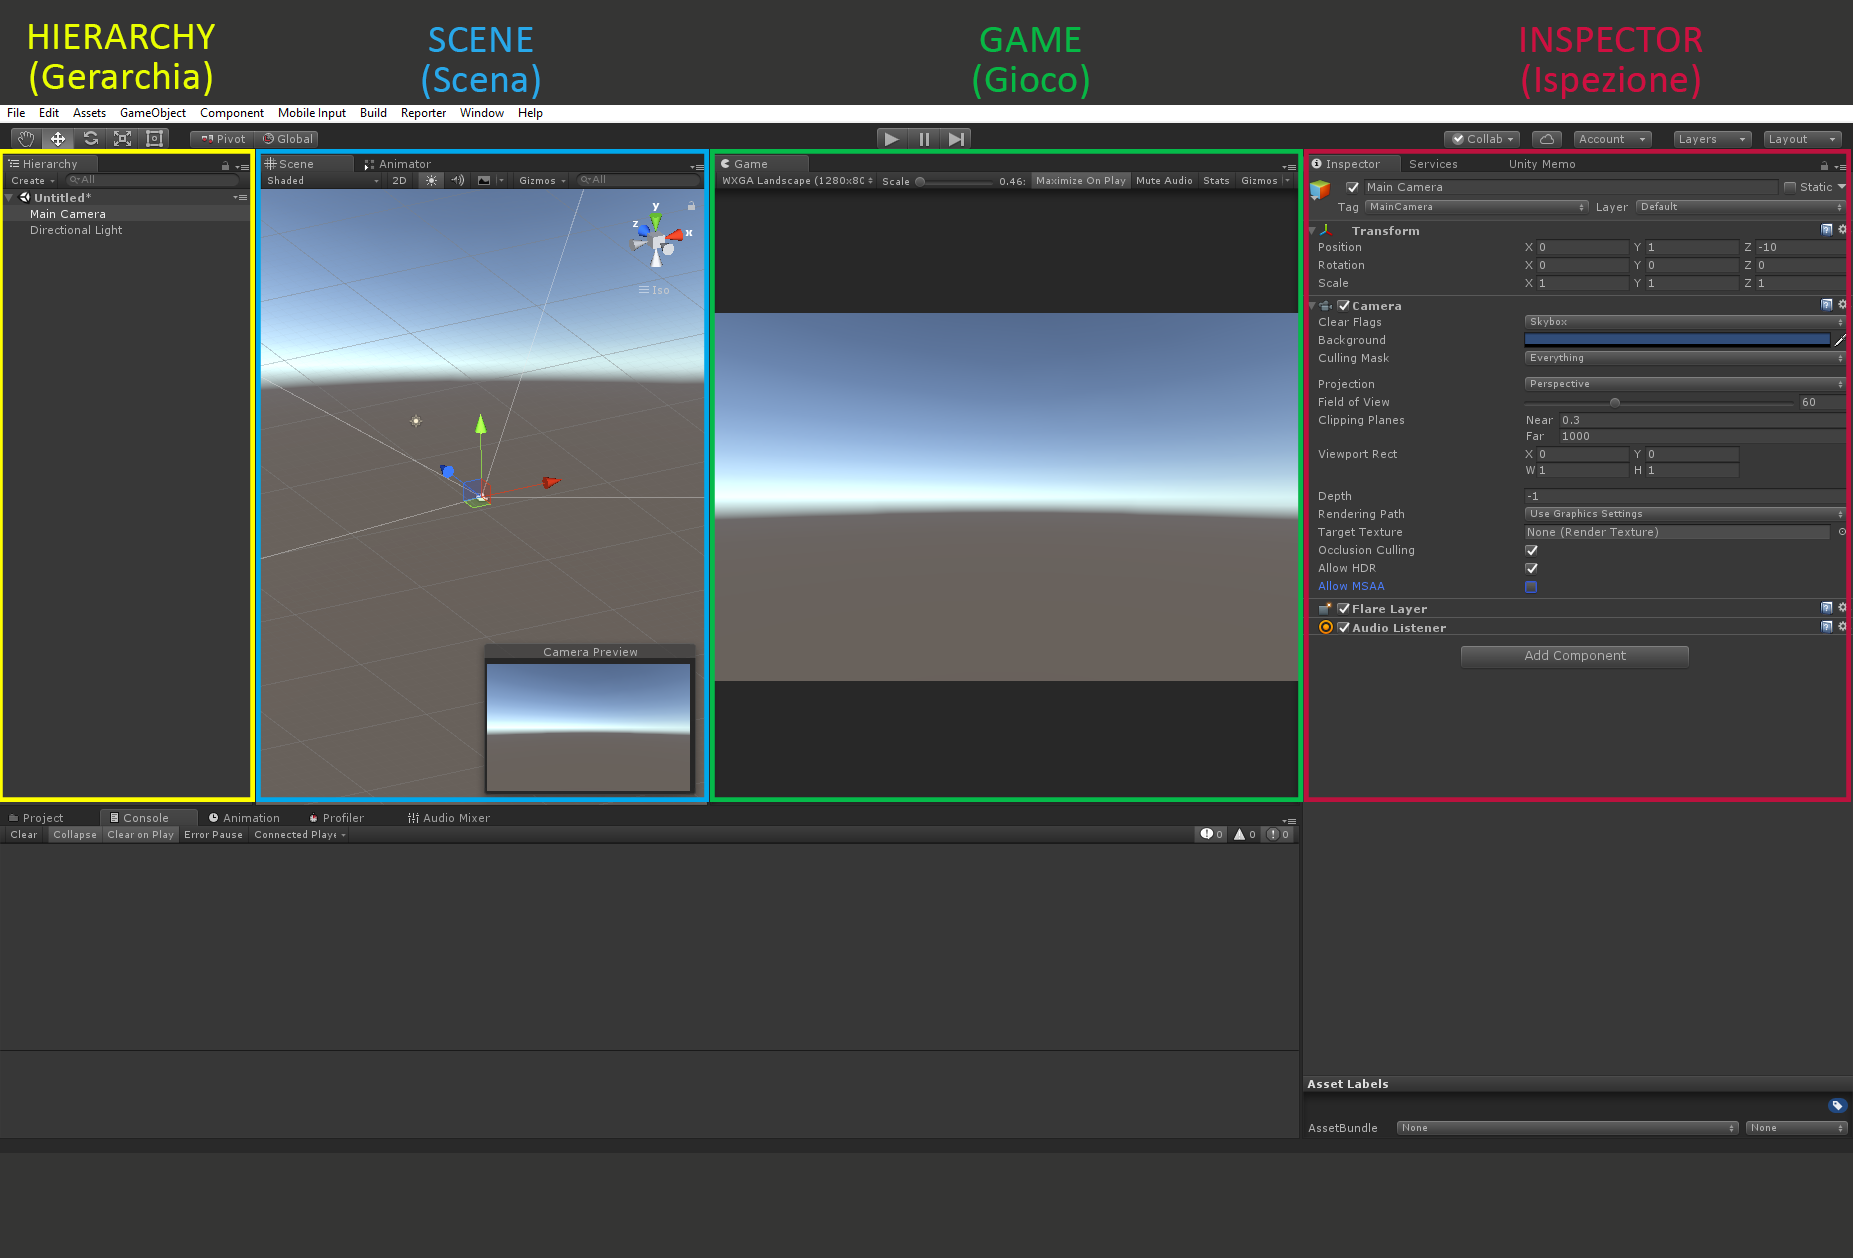
\includegraphics[width=0.8\linewidth]{image/unity}
		\caption{Schermate unity}
		\label{fig:unity}
	\end{figure}
	Questo motore di gioco mi ha permesso  di poter realizzare il gioco indipendentemente dalla piattaforma per poi andare a costruire la versione apposita, senza dovere effettuare nessuna modifica.
	Una funzione molto importante per questo progetto è stata la simulazione su dispositivo android, il quale mi ha permesso di poter provare l'applicativo direttamente sul mio telefono , e al contempo interagire e/o modificare la scena senza doverlo installare sul telefono.
    L'Asset Store, è una delle caratteristiche che ho trovato fondamentale, ovvero unity3D, mette a disposizione una serie di oggetti, pubblicati anche dall'utente, che permettono di tralasciare alcuni aspetti in modo da potersi concentrare su altro.
	I materiali presenti sul Asset Store vanno dai semplici oggetti 3D,script a veri e propri pacchetti.
	Al interno del Asset Store è possibile quindi trovare tutti gli elementi utili per poter sviluppare un gioco da zero, volendo anche gratuitamente.
	\subsection{Visual code}
	Visual code è un editor di codice usato in correlazione con unity 3D per la realizzazione degli script di gioco, figura:\ref{fig:visual_code}.
    Come già menzionato in precedenza, Visual Studio Code è un editor di codice sorgente sviluppato da Microsoft che ha guadagnato rapidamente popolarità tra gli sviluppatori. È gratuito, multipiattaforma e altamente personalizzabile grazie all'ampia gamma di estensioni disponibili attraverso il marketplace integrato.
	Una delle caratteristiche distintive di Visual Studio Code è la sua interfaccia utente pulita e intuitiva. L'editor utilizza una combinazione di barre degli strumenti, pannelli laterali e schede per fornire un accesso rapido alle funzionalità chiave.
	Un'altra caratteristica importante di Visual Studio Code è la sua capacità di supportare molteplici linguaggi di programmazione.
	\begin{figure}[H]
		\centering
		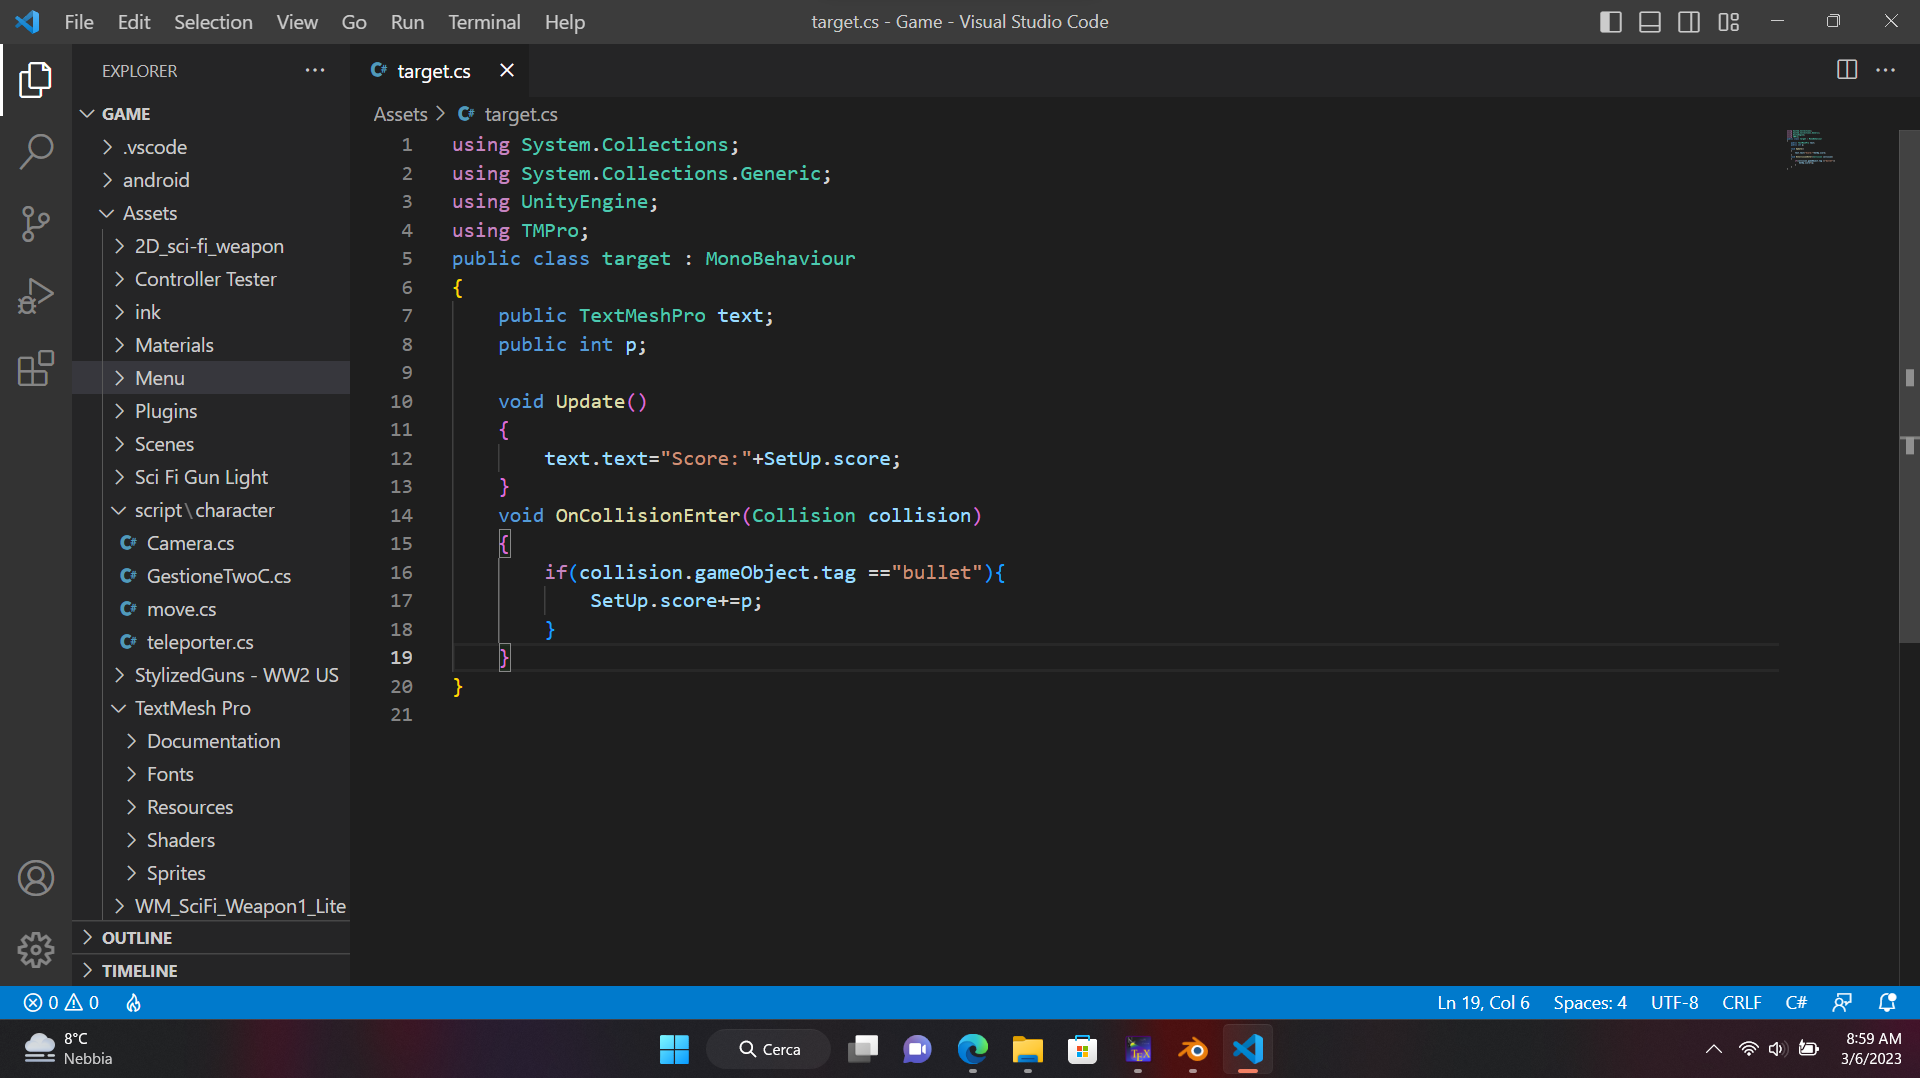
\includegraphics[width=0.8\linewidth]{image/visual_code}
		\caption{Esempio di script realizzato con visual code}
		\label{fig:visual_code}
	\end{figure}
	Le estensioni utilizzate in questo progetto riguardano principalmente l'interazione con unity 3D:
	\begin{itemize}
		\item Unity code snippets\cite{code-snippets}, usato per introdurre l'auto completamento.
		\item Unity tools\cite{UnityTools}, installato per poter consultare la documentazione in modo facile e dinamico. 
	\end{itemize}
	
	\chapter{Implementazione}
	In questo capitolo mi concentrerò sullo sviluppo del gioco, andando anche a descrivere i vari problemi che ho riscontrato.
	Ho deciso di utilizzare Unity 3D come motore di gioco, per l'interazione ho optato per il gamepad, in modo da poter interagire efficacemente con il mondo di gioco.
	Il seguente capitolo è stato diviso principalmente in tre parti:
	\begin{enumerate}
		\item Fase di prototipazione, in questa fase sono andato a definire i requisiti di progetto e la loro fattibilità, dopo aver fatto ciò, sono andato a sviluppare le componenti principali, il tutto è stato fatto all'interno di un ambiente di testing.
		\begin{figure}[H]
			\centering
			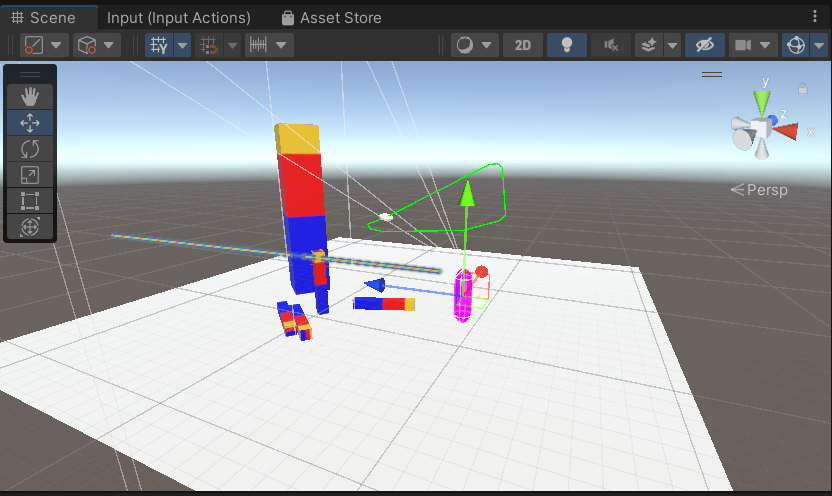
\includegraphics[width=0.8\linewidth]{image/protot}
			\caption{Scena prototipale}
			\label{fig:protot}
		\end{figure}
		\item Fase di sviluppo, dopo aver definito i vari requisiti ed aver sviluppato le componenti fondamentali, mi sono cimentato nella creazione effettiva dei vari livelli, in cui sono andato ad utilizzare le componenti sopra sviluppate.
		\item Problemi riscontati, in cui andrò ad esporre i principali problemi che ho dovuto risolvere.
	\end{enumerate}
	\section{Fase di prototipazione}
	Come detto in precedenza, in questa fase sono andato a definire le componenti principale del progetto:
	\begin{itemize}
		\item Visuale, in cui mi sono occupato di gestire due visualizzazioni differenti.
		\item Mappatura dei tasti, in cui ho definito i tasti utilizzati e le azioni a esse collegate.
		\item Menu, in cui ho implementato i menu di scelta con le relative finestre.
	\end{itemize}
	\subsection{Visuale}
	Per la visuale, la preoccupazione più grande è stata ideare un sistema che permettesse di differenziare le immagini dirette nei rispettivi occhi, per fare ciò ho usato due telecamere, poste all'interno di un oggetto, in cui è presente lo script \textit{Camera}, di cui discuterò più avanti.
	Le due telecamere sono state poste alla distanza interpupillare media, 62mm\cite{Distanza_occhi}.
	Come accennato prima, le telecamere mostrano oggetti diversi, ovvero, oltre al effetto dovuta alla distanza, utile per ricreare l'effetto tridimensionale, mi sono anche preoccupato di trovare uno stratagemma che mi permettesse di mostrare lo stesso oggetto in maniera differente, l'effetto trasparenza.
	L'effetto visivo desiderato è stato ricreato mediante la creazione dello script \textit{SetUp}, che sfrutta la funzionalità di Unity3D di poter duplicare gli oggetti identificati con il tag \textit{OcchioMalato}. Lo script utilizza il metodo \textit{Instantiate} per creare una copia dell'oggetto, a cui viene applicato un effetto di trasparenza modificandone il materiale. Infine, la copia trasparente viene mostrata all'occhio sano, mentre l'originale non trasparente viene mostrato all'occhio pigro. Quest'ultima parte è gestita dallo script \textit{GestioneTwoC}.
	Come detto in precedenza le due telecamere sono poste all'interno di un oggetto padre, il quale contiene lo script \textit{Camera}.
	Questo script mi permette di utilizzare il giroscopio del telefono in modo da poter regolare l'angolazione della visuale.
	Per l'integrazione del giroscopio all'interno del sistema ho utilizzato la classe \textit{Gyroscope}, il quale mi permette di ottenere diversi valori:
	\begin{itemize}
		\item attitude,	Restituisce l'orientamento nello spazio del dispositivo.
		\item enabled, Imposta o recupera lo stato di abilitazione del giroscopio.
		\item gravity, Restituisce il vettore dell'accelerazione di gravità.
		\item rotationRate,	Restituisce la velocità di rotazione misurata dal giroscopio.
		\item rotationRateUnbiased,	Restituisce il tasso di rotazione elaborato.
		\item updateInterval, Imposta o recupera l'intervallo di misurazione del giroscopio in secondi.
		\item userAcceleration,	Restituisce l'accelerazione che l'utente fornisce al dispositivo.
	\end{itemize}
	Nel mio caso sono andato ad usare \textit{rotationRate}, figura:\ref{fig:code_giro}
	\begin{figure}[H]
		\centering
		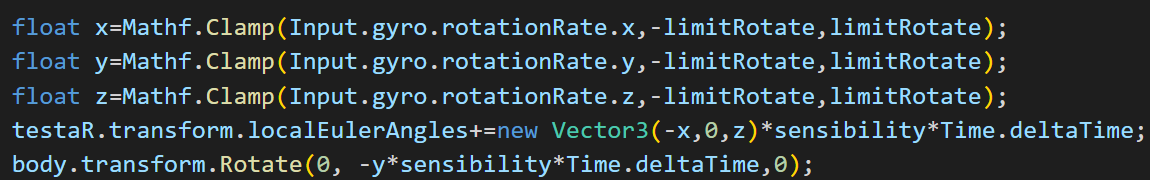
\includegraphics[width=1\linewidth]{image/codice_giro}
		\caption{Codice usato}
		\label{fig:code_giro}
	\end{figure}
	Per evitare movimenti troppo bruschi, ho limitato la massima e minima velocità di rotazione, attraverso \textit{limitRotate}.
	\begin{displaymath}
		-limtiRotate  \leq X \leq limitRotate
	\end{displaymath}
	\subsection{Mappatura}
    Per la mappatura, mi sono preoccupato di associare ogni tasto ad una specifica funzione in modo da ricreare una facile ergonomia. Questo permette di riconoscere i tasti principali senza l'utilizzo della vista durante l'esperienza, in quanto è richiesto l'uso del cardboard. Di seguito, nella figura \ref{fig:gamepad_tasti}, riporto il layout dei tasti con le funzioni associate. Ho raggruppato la presentazione in due macro gruppi:
	Ho raggruppato la presentazione in 2 macro gruppi:Azioni personaggio e Navigazione menu.
	\begin{figure}[H]
		\centering
		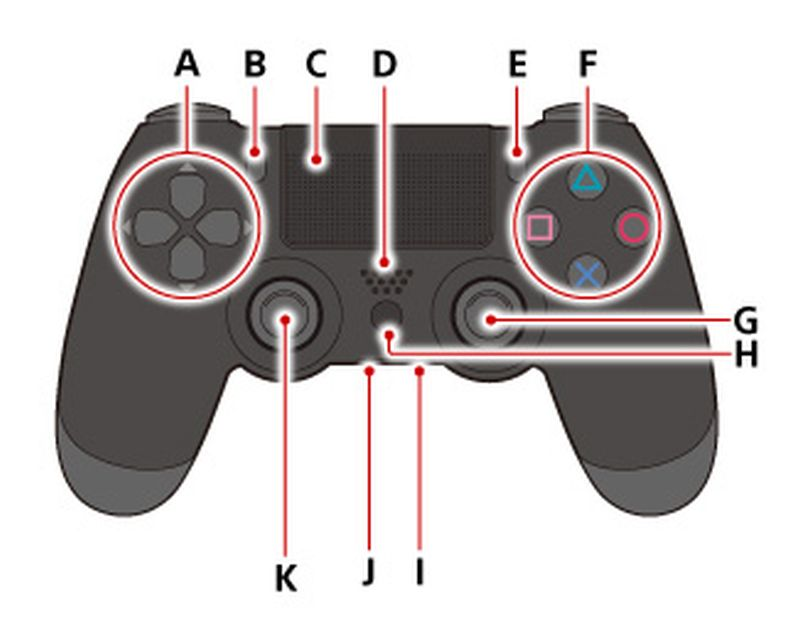
\includegraphics[width=0.6\linewidth]{image/gamepad_tasti}
		\caption{Mappatura tasti}
		\label{fig:gamepad_tasti}
	\end{figure}
	Per il macro gruppo, azioni del personaggio, vado ad elencare tutte le possibilità date al paziente, per navigare e interagire con i vari livelli dati a disposizione.
	\begin{itemize}
		\item Movimento tridimensionale.\textit{Stick G}
		\item Teletrasporto.\textit{Stick K}
		\item Sparo.\textit{Dorsale RT}
		\item Accucciarsi,Abbassarsi.\textit{Tasto stick G}
		\item Voltarsi.\textit{RB+Stick G}
		\item Sporgesi.\textit{D Pad:A Tasti orizzontali}
		\item Riposizionamento telecamera.\textit{Tasto triangolo}
	\end{itemize}
	Per il macro gruppo, navigazione dei menu, vado ad elencare l'insieme dei tasti attui ad utilizzare correttamente il menu.
	\begin{itemize}
		\item Apertura e Chiusura:\textit{Tasto E}
		\item Pagina precedente:\textit{Tasto B}
		\item Navigazione opzioni.\textit{D Pad Tasti verticali}
		\item Clicca e salva:\textit{Tasto quadrato}
	\end{itemize}
	Come si può evincere, vi sono tasti non assegnati, questo implica la possibilità di espandere le funzionalità del gioco mediante l'implementazione non solo di nuovi livelli ma anche di nuove funzioni e azioni.
	\subsection{Menu}
	Nella creazione dei menu, mi sono concentrato a cercare un sistema che rispettasse il concetto di stereogramma\cite{Stereogramma}. Ho notato che i classici strumenti di Unity per la creazione dei menu non permettono di rispettare il principio fondamentale dell'immagine stereoscopica. In questo tipo di immagini, lo stesso oggetto - in questo caso, il menu - deve essere osservato con una variazione di prospettiva per creare l'effetto tridimensionale.
	Per ovviare a ciò, sono andato a ricreare il menu nel mondo di gioco, in modo che venisse ripreso dalle due telecamere, con differente prospettiva, figura:\ref{fig:menu_scena}.
	\begin{figure}[h]
		\centering
		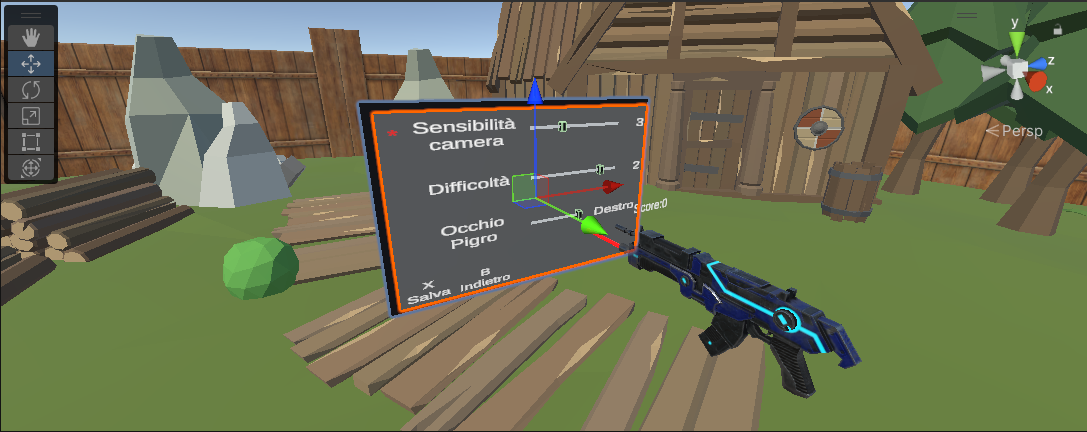
\includegraphics[width=0.6\linewidth]{image/menu_scena}
		\caption{Vista del menu nella finestra \textit{Scene}}
		\label{fig:menu_scena}
	\end{figure}
	In questo modo l'effetto ottenuto, figura:\ref{fig:menu_simulator}, rispetta il principio citato prima.
	\begin{figure}[h]
		\centering
		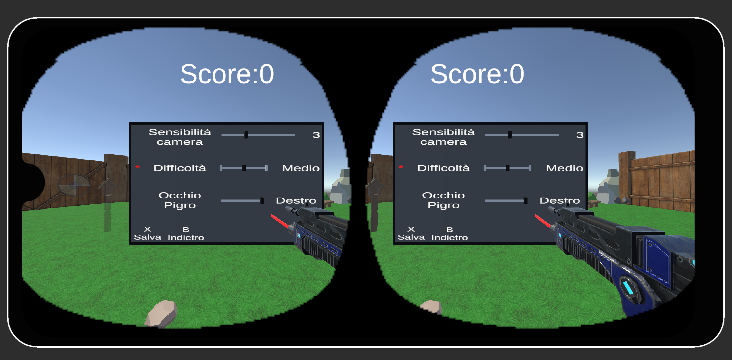
\includegraphics[width=0.6\linewidth]{image/menu_simulatore}
		\caption{Vista del menu nella finestra \textit{simulator}}
		\label{fig:menu_simulator}
	\end{figure}
	Dopo aver ricreato la schermata del menu sono andato ad inserire le impostazione che ho ritenuto più importanti
	\begin{itemize}
		\item Sensibilità camera, in cui vado ad inserire la velocità con cui la visuale cambia in relazione al giroscopio del telefono.
		\item Difficoltà, in questo caso definisco il grado di trasparenza. 
		\item Occhio Pigro, che mi permette di settare qual'è l'occhio pigro, in modo da poter cambiare la renderizzazione del gioco.
	\end{itemize}
    Il menu è stato realizzato grazie allo script principale denominato \textit{Choice}, il quale è stato esteso dallo script \textit{Setting}, il quale si occupa della gestione degli oggetti interagibili presenti nel menu. Ogni oggetto presente nel menu estende a sua volta lo script \textit{Option}, il quale contiene l'attributo \textit{status} che indica se l'oggetto è stato selezionato o meno. In questo modo, basta guardare lo status dell'oggetto per sapere se l'azione associata ad esso deve essere eseguita, ad esempio cliccare su un pulsante o cambiare un'impostazione, in questo modo, l'azione che vado ad eseguire può essere di qualsiasi tipo.
	\begin{figure}[h]
		\centering
		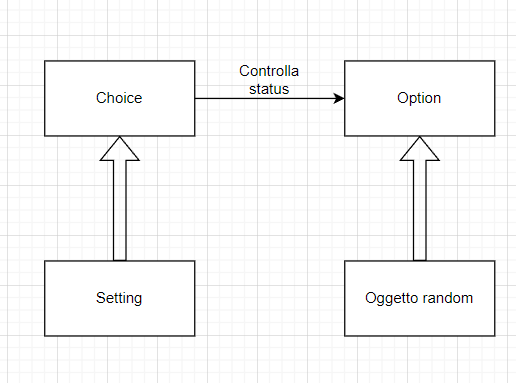
\includegraphics[width=0.6\linewidth]{image/funzionamento menu}
		\caption{Schema script}
		\label{fig:menu_funzionamento}
    \end{figure}
	\section{Fase di sviluppo}
	Dopo aver completato la fase di progettazione e creazione dei vari componenti del gioco, mi sono concentrato sulla fase di sviluppo vera e propria. Durante questa fase, ho lavorato alla creazione dei singoli livelli del gioco, con l'obiettivo di rendere l'esperienza di gioco il più coinvolgente possibile. In questa sezione, descriverò il processo di sviluppo dei vari livelli.
	Per prima cosa, sono andato ad importare i vari Asset, edifici, oggetti, ecc, in modo da potermi focalizzare su altri aspetti che ho reputato più importanti.
	Gli asset che ho utilizzato sono:
	\begin{itemize}
		\item Rocce\cite{Rock_asset}
		\item Asset medievale\cite{Pack_asset}, contenente edifici, alberi e oggetti medievali. 
		\item Muri\cite{Wall_asset}, contente i vari muri che circondano ogni livello.
		\item Curva di Bézier\cite{Pack_asset}, il quale mi ha permesso di ricreare i Target in movimento.
		\item Controller Test\cite{Controller_test}, Asset utilizzato per la mappatura, questione approfondita più avanti.
		\item Arma\cite{pistola}, contiene l'asset che ho utilizzato come emettitore del raycast,precisamente all'interno del progetto è denominato \textit{GunHeavy} e svolge la funzione di arma.
	\end{itemize}
	Dopo aver selezionato i singoli asset, sono andato ad assemblare il personaggio giocante.
	\subsection{Personaggio}
	Il personaggio, come è possibile intuire è l'elemento principale di tutta l'esperienza, per questo motivo andrò a descriverne i singoli componenti.
	\begin{itemize}
		\item Camera, in cui vado a ruotare e/o muovere l'oggetto \textit{testa}, contenente le due telecamere.
		\item GestioneTwo, dove mi sono concentrato sulla gestione delle due telecamere del gioco, ricreando l'effetto trasparenza e di profondità.
		\item Move, è uno script che ho sviluppato per gestire il movimento all'interno del gioco,questo script è stata fondamentale per garantire un'esperienza di gioco coinvolgente e immersiva.
		\item Shoot, riguarda l'implementazione di un'azione fondamentale del gioco, il quale permette ai giocatori di raccogliere punti sparando ai Target disseminati nella mappa
		\item Teleporter, è uno script che ho creato per gestire il teletrasporto all'interno del gioco. Questo elemento è stato implementato per garantire una seconda opzione di movimento, nel caso in cui il motion sickness\cite{mottion_sickness} dovesse influenzare negativamente l'esperienza di gioco degli utenti.
	\end{itemize}
	Gli script sopra citati, vengono organizzati seguendo uno schema gerarchico, figura:\ref{fig:script_character}, essi compongono il personaggio, il componente più importante del gioco.
	\begin{figure}[H]
		\centering
		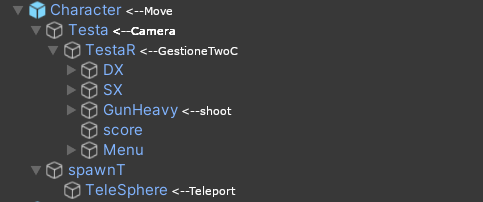
\includegraphics[width=0.8\linewidth]{image/script_character}
		\caption{Organizzazione script}
		\label{fig:script_character}
	\end{figure}
	Oltre agli elementi sopra citati, sono contenuti all'interno del personaggio altri elementi, tra cui:
	\begin{itemize}
		\item DX e SX, le due telecamere usate per ricreare l'effetto stereoscopica.
		\item score, il quale visualizza il punteggio.
		\item Menu, implementa il sistema menu, descritto nel paragrafo precedente.
		\item spawnT, consente di impostare la posizione di origine dell'oggetto chiamato \textit{TeleSphere}, il quale può essere spostato in modo che funga da punto di riferimento per il teletrasporto.
	\end{itemize}
	L'oggetto \textit{GunHeavy} contiene lo script \textit{shoot} come mostrato nella figura \ref{fig:script_character}. Questo script gestisce l'azione di sparare utilizzando la classe Raycast di Unity 3D. La classe Raycast permette di emettere un raggio dalla posizione dell'oggetto in gioco e di determinare se colpisce altri oggetti nella scena. Questa funzione è stata utilizzata per permettere al giocatore di sparare ai vari target guadagnando punti.
	Quando il Raycast colpisce i Target, attiva una funzione all'interno degli stessi che permette di conteggiare i punti ottenuti dal giocatore, chiamata hit.\\
	Dopo aver costruito il personaggio giocante, sono andato a creare il terreno di gioco, disseminando rocce, edifici e oggetti di scena.
	\subsection{Mappa}
	Uno degli aspetti fondamentali del progetto è stato il posizionamento e la scelta degli oggetti \textit{OcchioMalato}, poiché l'obiettivo principale è quello di stimolare efficacemente l'occhio pigro, costringendo il paziente a prestare attenzione agli elementi del paesaggio. Legato a questo, ho disseminato ogni livello con un determinato numero di Target fissi e/o in movimento che sono essenziali per il prosieguo del gioco e della terapia. Per quanto riguarda i Target, essi sono composti da un singolo script chiamato \textit{target} nel caso degli statici, mentre per quelli in movimento, mi sono servito di uno script aggiuntivo che ricrea le curve di Bézier \cite{Pack_asset}.
	Le curve di Bézier \cite{Path_asset}, utilizzate principalmente in ambito grafico e di progettazione assistita dal computer (CAD), sono state utilizzate in questo caso per delineare il percorso che i vari Target devono seguire. Queste curve sono particolarmente utili per creare forme e traiettorie fluide e precise utilizzando un insieme di punti di controllo. Le curve sono state rappresentate in verde nella figura: \ref{fig:mappa}.
	\begin{figure}[H]
		\centering
		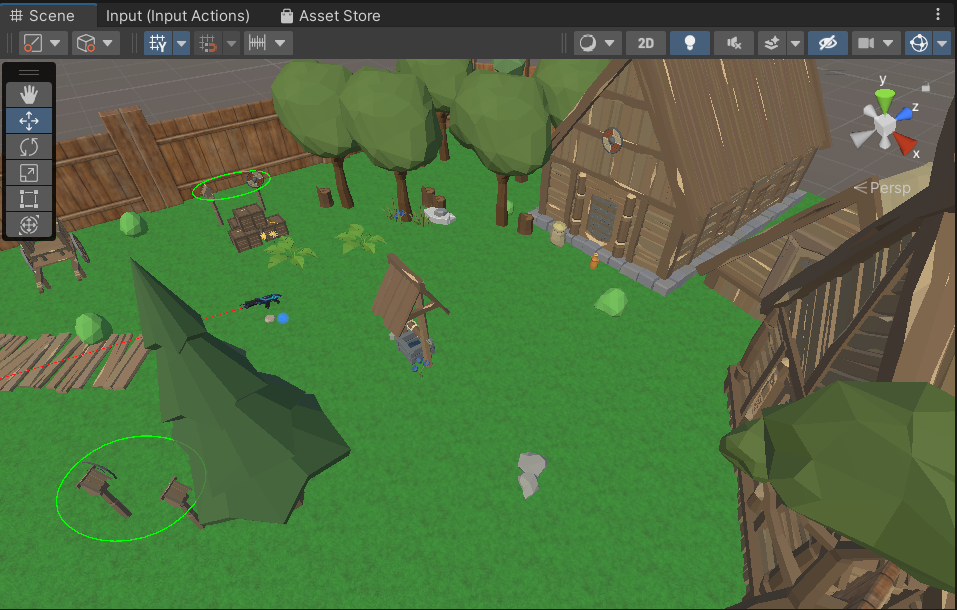
\includegraphics[width=0.6\linewidth]{image/mappa}
		\caption{Secondo livello}
		\label{fig:mappa}
	\end{figure}
	Nello script del Target, oltre a definire la funzione \textit{hit} scatenata dal Raycast, è stata implementata anche la creazione dell'oggetto \textit{fly score} attraverso il metodo \textit{Instantiate}, che sostituisce il target al momento dell'attivazione della funzione \textit{hit}. All'interno di questo oggetto è stato implementato uno script che crea un effetto visivo in cui il punteggio del target colpito vola verso l'alto rimpicciolendosi gradualmente, come mostrato in figura: \ref{fig:fly score}. Inoltre, è stata utilizzata una funzione coseno per generare una leggera turbolenza al fine di rendere l'effetto più dinamico.
	\begin{figure}[H]
		\centering
		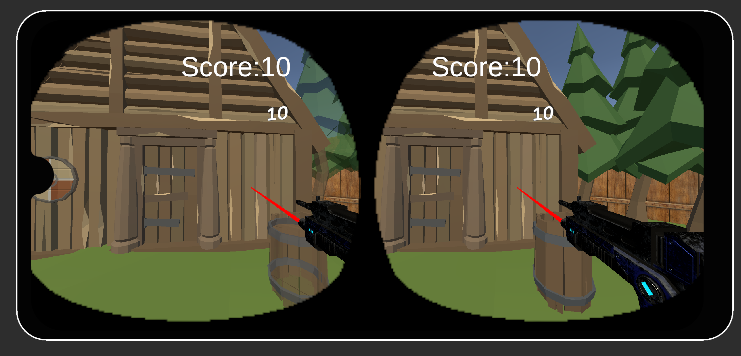
\includegraphics[width=0.6\linewidth]{image/fly score}
		\caption{Esempio fly score}
		\label{fig:fly score}
	\end{figure}
	\subsubsection{Portale}
   Come accennato in precedenza, c'è un portale presente su ogni mappa che, una volta attraversato, consente di accedere al livello successivo. Questo portale è stato realizzato utilizzando uno sprite raffigurante un cerchio nero adornato con alcune pietre in movimento che permettono di simulare l'effetto di un buco nero, come mostrato in figura: \ref{fig:portale}. 
  \begin{figure}[H]
  	\centering
  	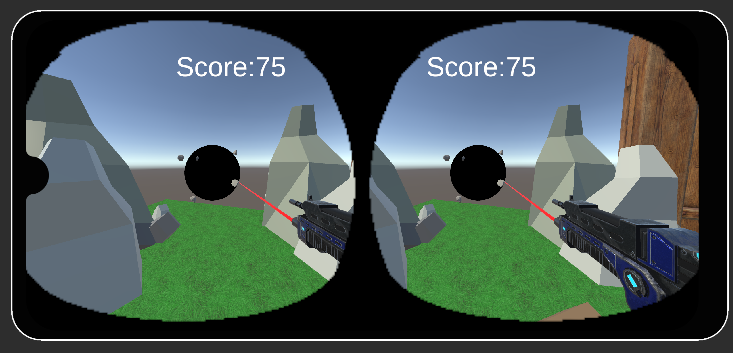
\includegraphics[width=0.6\linewidth]{image/portale}
  	\caption{Portale livello 3}
  	\label{fig:portale}
  \end{figure}
   L'innovativo effetto grafico utilizzato è stato studiato per rendere l'esperienza di gioco più fluida ed entusiasmante, evitando quei cambi di livello bruschi che potrebbero diminuire la soddisfazione del giocatore durante la partita. Una volta completato il livello, il giocatore si sentirà ancora più motivato a proseguire grazie alla sensazione di avventura e originalità conferita dall'effetto grafico. Questo è fondamentale per convincere il paziente a continuare con la terapia ludica, garantendo una maggiore efficacia nell'ottenere i risultati desiderati.
	\section{Problemi}
    In questo paragrafo elencherò le limitazioni e le forzature che ho introdotto nel progetto per garantirne la stabilità. Come già accennato in precedenza, capitolo:\ref{chap:cardboard_motivi}, l'utilizzo del Cardboard mi ha fornito un set di tecnologie molto utili, ma ha anche comportato una limitazione tecnica significativa. Lo smartphone utilizzato con il Cardboard non è in grado di elaborare immagini troppo complesse, il che mi ha costretto a scegliere uno stile low poly per gli asset gioco. Questa limitazione si può anche osservare dagli alberi scelti i quali non presentano foglie ma chiome stilizzate, figura:\ref{fig:low_hight}.
	\begin{figure}[H]
		\centering
		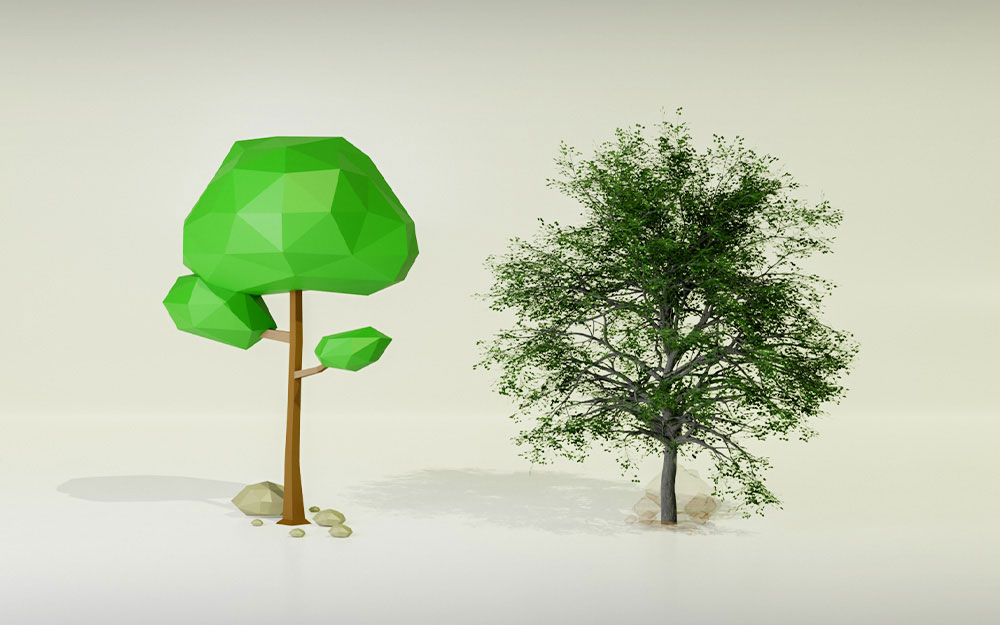
\includegraphics[width=0.6\linewidth]{image/low_hight}
		\caption{Albero low poly contro hight poly.Fonte:\cite{low_high}}
		\label{fig:low_hight}
	\end{figure}
   In relazione a ciò, parlerò della trasparenza, che è stata ampiamente discussa nei paragrafi precedenti e che comporta la duplicazione degli oggetti identificati come \textit{OcchioMalato}, modificandone il materiale. L'operazione sopra descritta implica che lo smartphone dovrà renderizzare e tenere in memoria, nel peggior dei casi, il doppio degli elementi. Ciò implica che bisogna scegliere saggiamente a quali oggetti impostare il tag "OcchioMalato" per evitare di sovraccaricare il telefono.
   Infine, per chiudere il discorso cardboard, andrò a parlare della limitazione che influisce maggiormente sull'immersività del gioco, ovvero la limitazione dei gradi di libertà dell'oggetto "Testa", il quale è responsabile di orientare le due telecamere. Ho deciso di limitare la rotazione sull'asse z in quanto, dopo svariati test, mi sono accorto che essa causava problemi di mancata sincronizzazione tra il cardboard e il gioco.\\\\
   Un altro problema, non correlato al cardboard, riguarda la mappatura dei comandi. Inizialmente, non avevo trovato la mappatura del gamepad utilizzato, il che significava che non avevo informazioni sui codici associati ad ogni tasto. Per risolvere il problema della mappatura dei comandi, ho utilizzato un asset chiamato Controller test \cite{Controller_test}, reperibile sull'Asset Store di Unity3D. Dopo averlo installato sul telefono, l'asset sopra citato mi ha permesso di visualizzare i codici associati ai tasti e di mapparli correttamente in Unity3D, figura:\ref{fig:controller_test}. In questo modo, ho risolto il problema della mappatura. \ref{fig:controller_test}.
	\begin{figure}[H]
		\centering
		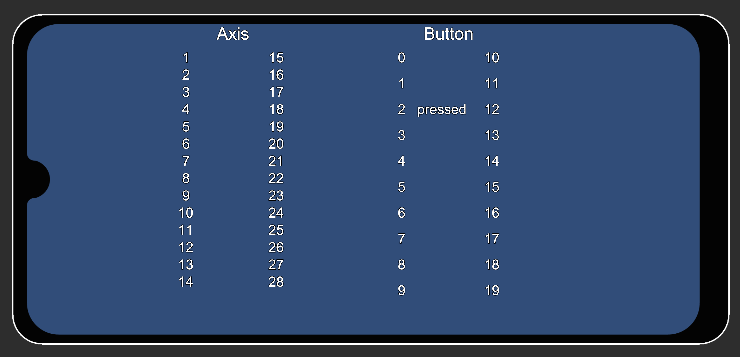
\includegraphics[width=0.7\linewidth]{image/controller_test}
		\caption{Prova controller test, per tasto X}
		\label{fig:controller_test}
	\end{figure}
	Grazie a questo strumento, sono stato in grado di associare i codici dei singoli tasti alle corrispondenti azioni di gioco.
	\chapter{Conclusioni e Sviluppi futuri}
	In conclusione, la creazione di un'applicazione per il trattamento dell'ambliopia rappresenta un importante passo avanti nella lotta contro questa patologia visiva. Grazie alla combinazione di tecnologie alla portata di tutti, l'applicazione proposta si propone di aiutare i pazienti affetti da ambliopia a migliorare la loro acuità visiva e la loro qualità di vita. Tuttavia, come tutte le tecnologie sanitarie, anche questa applicazione necessita di essere testata ed evoluta nel tempo, al fine di garantire la massima efficacia e sicurezza per i pazienti.\\\\
	
	Uno sviluppo futuro potrebbe riguardare l'implementazione di un sistema multiplayer, il quale permetterebbe ai pazienti di sentirsi meno soli durante questo percorso, aumentando così l'esposizione al trattamento. Inoltre, considerando le limitazioni emerse durante lo sviluppo del progetto riguardanti l'utilizzo del cardboard, sarebbe interessante sviluppare questa applicazione per un visore che non abbia le limitazioni citate in precedenza. Ciò potrebbe comportare un ulteriore miglioramento dell'esperienza utente e dei risultati ottenuti dal trattamento. Inoltre, l'utilizzo delle VR controller gun potrebbe essere un altro interessante sviluppo, in quanto potrebbero aumentare il senso di immersione dell'utente all'interno dell'esperienza VR. Ciò potrebbe portare ad un ulteriore coinvolgimento dell'utente nel trattamento e potenzialmente migliorare i risultati a lungo termine.\\\\
	
	In sintesi, l'applicazione per il trattamento dell'ambliopia rappresenta un'importante innovazione tecnologica nel campo della diagnostica e cura delle patologie visive, e ha il potenziale per aiutare molti pazienti a migliorare la loro acuità visiva.
	
    
	\bibliographystyle{unsrt}
	\bibliography{./reference/r_web.bib,./reference/art.bib}	

\end{document}